\documentclass[spanish]{article}                 % Tipo de documento
\usepackage[paperheight=30in, paperwidth=120in]{geometry}
\usepackage[T1]{fontenc}                         % Codificación
\usepackage[utf8]{inputenc}
\usepackage[spanish, activeacute]{babel}         % Idioma español
\usepackage{newtxtext}
\usepackage{charter} % Fuente
\decimalpoint{}

\usepackage{amsmath, amsthm, amssymb}            % Entornos y símbolos ams
\numberwithin{equation}{section}                 % Numeración de ecuaciones
\newtheorem{teorema}{Teorema}[section]           % Teoremas y su numeración
\newtheorem{corolario}[teorema]{Corolario}
\newtheorem{lema}[teorema]{Lema}
\newtheorem{proposición}[teorema]{Proposición}
\theoremstyle{definition}
\newtheorem{definición}[teorema]{Definición}
\newtheorem{problema}{Problema}[section]
\newtheorem{solución}{Solución}

\usepackage[italic]{esdiff}                      % Derivadas
\usepackage{mathtools}

\usepackage[]{graphicx}
\usepackage{subfig}
                                                      % Operadores
\DeclarePairedDelimiter\abs{\lvert}{\rvert}           % Valor absoluto
\DeclarePairedDelimiter\norm{\lVert}{\rVert}          % Normas
\newcommand{\argmin}{\mathop{\mathrm{argmin}}\limits} % ArgMin
\newcommand{\argmax}{\mathop{\mathrm{argmax}}\limits} % ArgMax
\newcommand*\dif{\mathop{}\!\mathrm{d}}               % Diferencial para integrales

\title{sASD}
\author{Eduardo Alexis Romo Almazán}
% \date{}

%%%%%%%%%%%%%%%%%%%%%%%%%%%%%%%%%%%%%%%%%%%%%%%%%%%%%%%%%%%%%%%%%%%%%%%
%                              Documento                              %
%%%%%%%%%%%%%%%%%%%%%%%%%%%%%%%%%%%%%%%%%%%%%%%%%%%%%%%%%%%%%%%%%%%%%%%
\begin{document}
\maketitle

\begin{figure}
    \begin{tabular}{cccccccccccccccc}
        \subfloat[Real rank: 50]{\includegraphics{../House30/pexels-photo-462358__50_low_rank.png}}     &
        \subfloat[Masked]{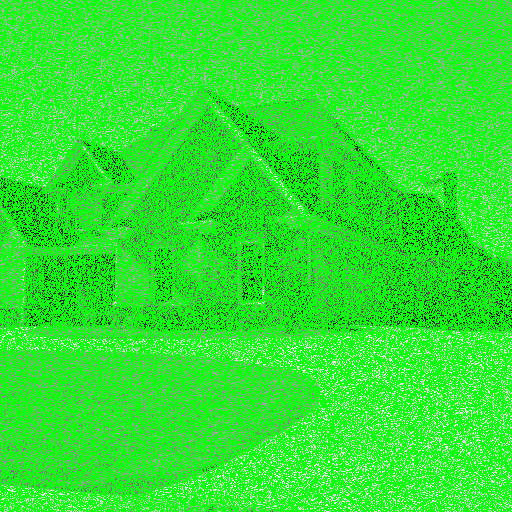
\includegraphics{../House30/pexels-photo-462358__masked.png}}            &
        \subfloat[Rank: 10]{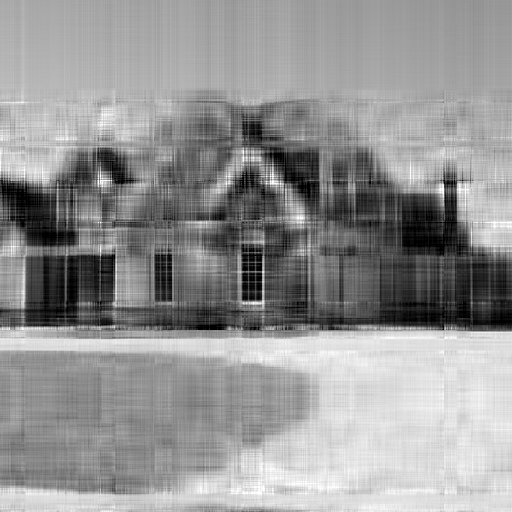
\includegraphics{../House30/pexels-photo-462358__50_10_30_approx.png}} &
        \subfloat[Rank: 20]{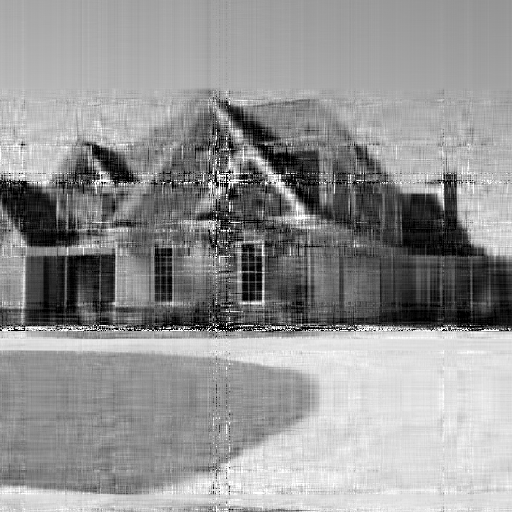
\includegraphics{../House30/pexels-photo-462358__50_20_30_approx.png}} &
        \subfloat[Rank: 30]{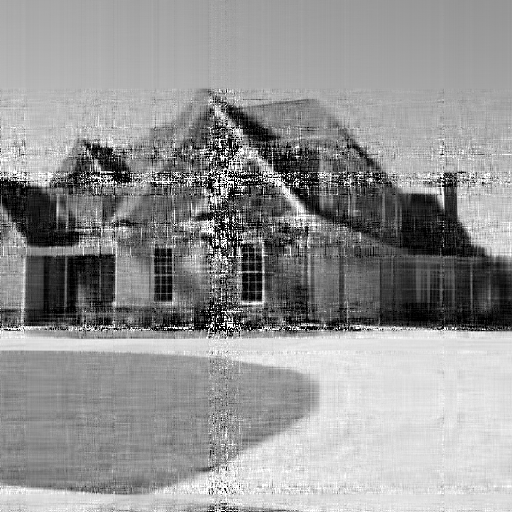
\includegraphics{../House30/pexels-photo-462358__50_30_30_approx.png}} &
        \subfloat[Rank: 40]{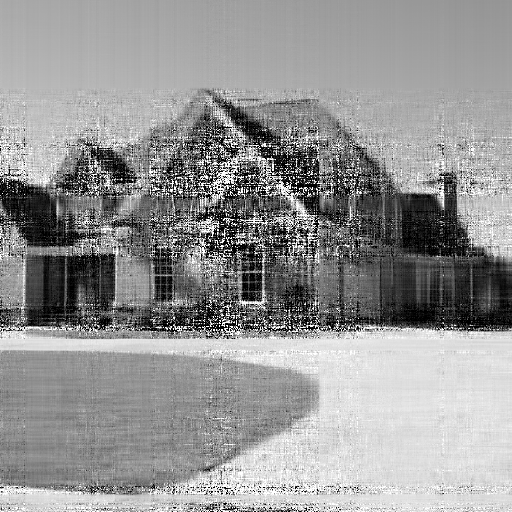
\includegraphics{../House30/pexels-photo-462358__50_40_30_approx.png}} &
        \subfloat[Rank: 50]{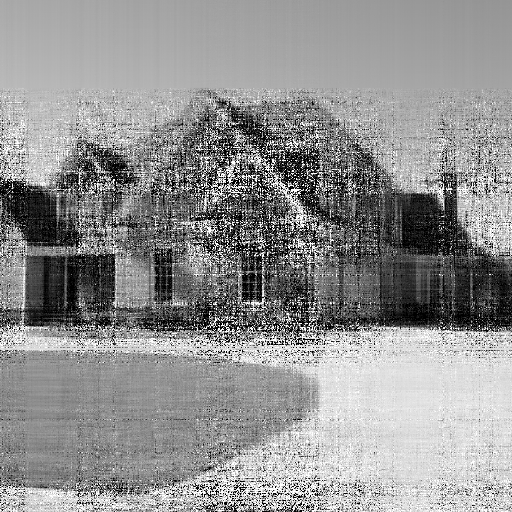
\includegraphics{../House30/pexels-photo-462358__50_50_30_approx.png}} &
        \subfloat[Rank: 60]{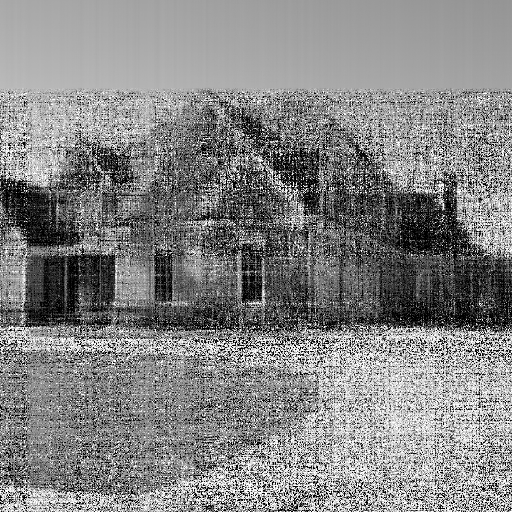
\includegraphics{../House30/pexels-photo-462358__50_60_30_approx.png}} &
        \subfloat[Rank: 70]{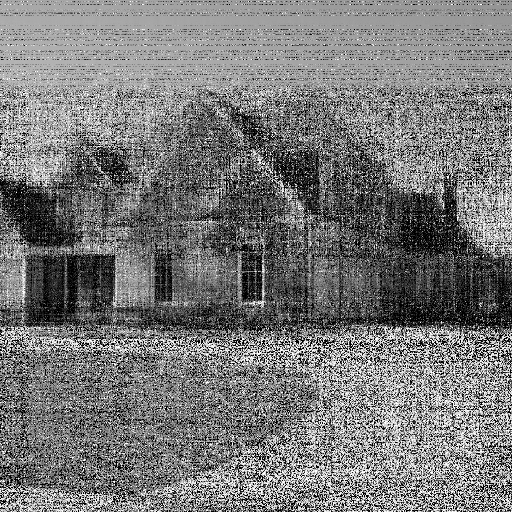
\includegraphics{../House30/pexels-photo-462358__50_70_30_approx.png}} &
        \subfloat[Rank: 80]{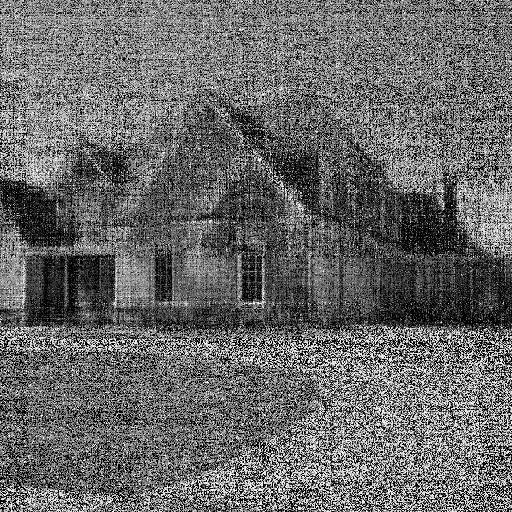
\includegraphics{../House30/pexels-photo-462358__50_80_30_approx.png}} &
        \subfloat[Rank: 90]{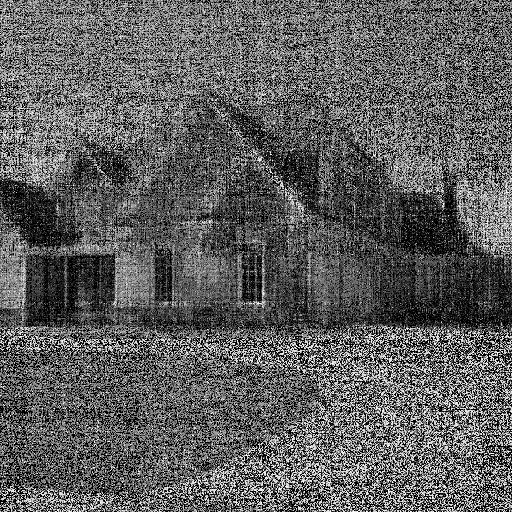
\includegraphics{../House30/pexels-photo-462358__50_90_30_approx.png}} &
        \subfloat[Rank: 100]{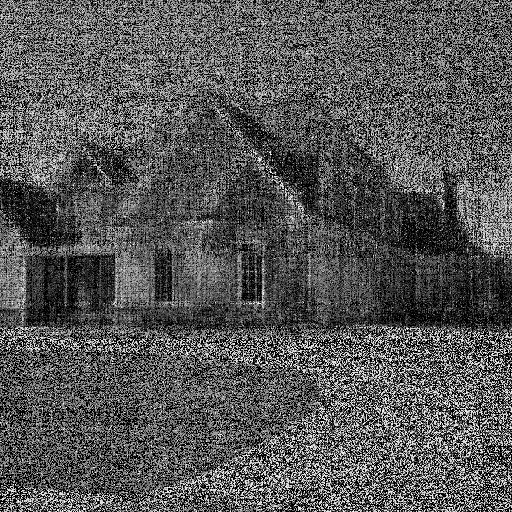
\includegraphics{../House30/pexels-photo-462358__50_100_30_approx.png}} \\
        \subfloat[Real rank: 50]{\includegraphics{../House40/pexels-photo-462358__50_low_rank.png}}     &
        \subfloat[Masked]{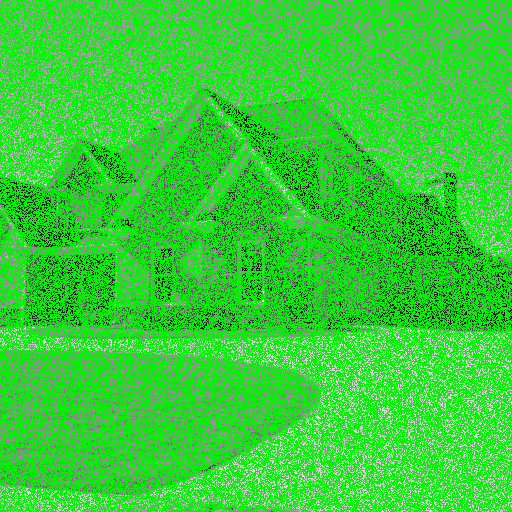
\includegraphics{../House40/pexels-photo-462358__masked.png}}            &
        \subfloat[Rank: 10]{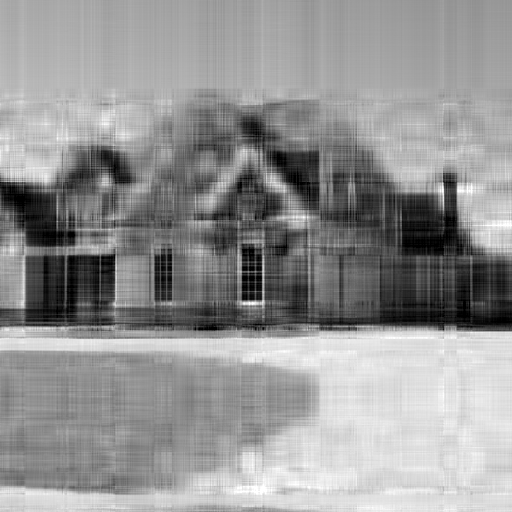
\includegraphics{../House40/pexels-photo-462358__50_10_40_approx.png}} &
        \subfloat[Rank: 20]{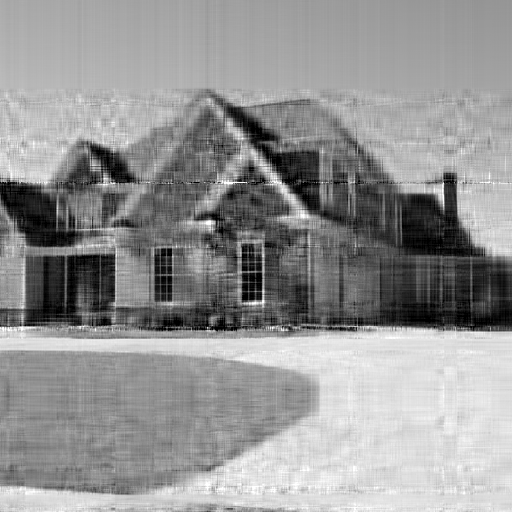
\includegraphics{../House40/pexels-photo-462358__50_20_40_approx.png}} &
        \subfloat[Rank: 30]{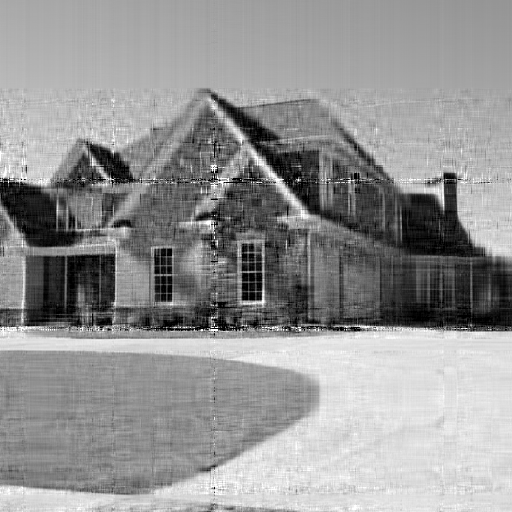
\includegraphics{../House40/pexels-photo-462358__50_30_40_approx.png}} &
        \subfloat[Rank: 40]{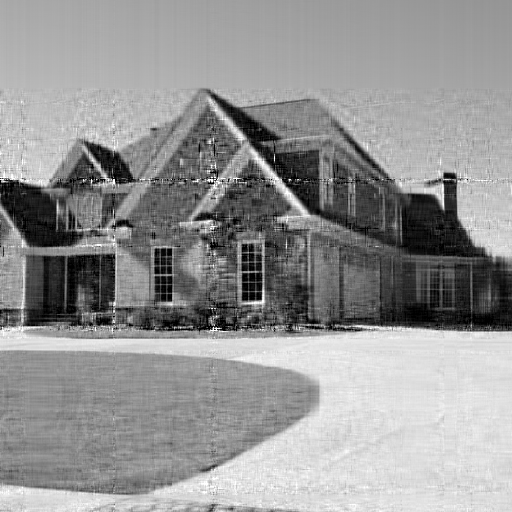
\includegraphics{../House40/pexels-photo-462358__50_40_40_approx.png}} &
        \subfloat[Rank: 50]{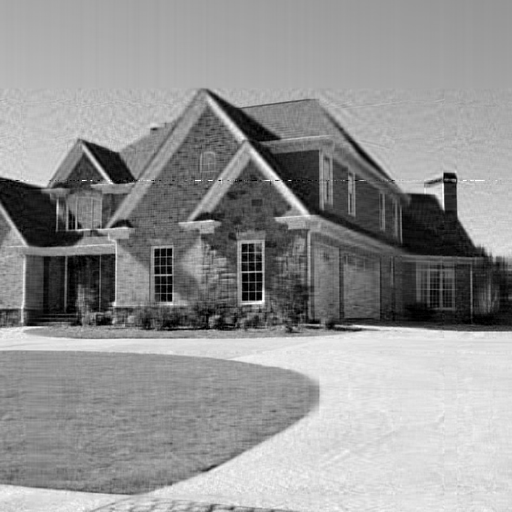
\includegraphics{../House40/pexels-photo-462358__50_50_40_approx.png}} &
        \subfloat[Rank: 60]{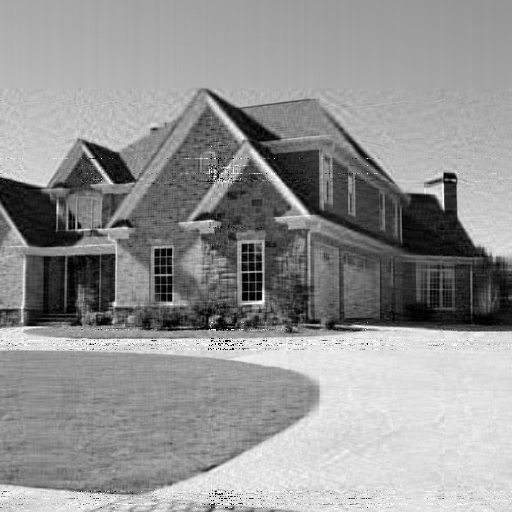
\includegraphics{../House40/pexels-photo-462358__50_60_40_approx.png}} &
        \subfloat[Rank: 70]{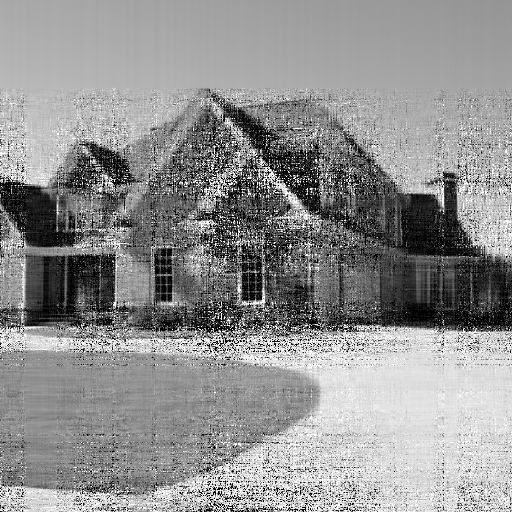
\includegraphics{../House40/pexels-photo-462358__50_70_40_approx.png}} &
        \subfloat[Rank: 80]{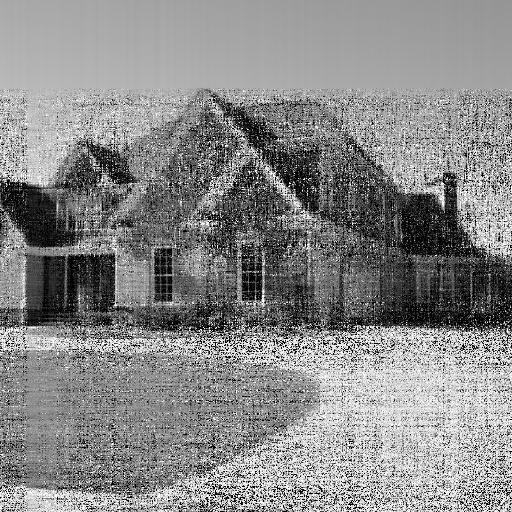
\includegraphics{../House40/pexels-photo-462358__50_80_40_approx.png}} &
        \subfloat[Rank: 90]{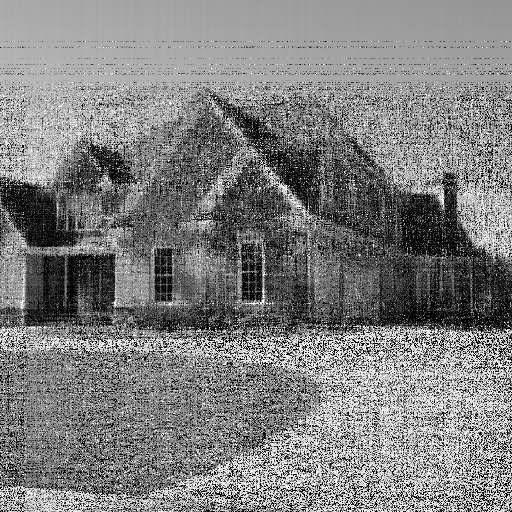
\includegraphics{../House40/pexels-photo-462358__50_90_40_approx.png}} &
        \subfloat[Rank: 100]{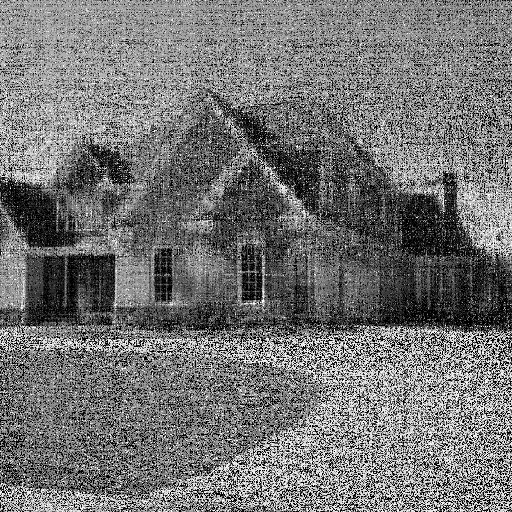
\includegraphics{../House40/pexels-photo-462358__50_100_40_approx.png}}
    \end{tabular}
    \caption{4 x 4}
\end{figure}

\end{document}
